\documentclass[12pt,compress,aspectratio=169]{beamer}
\usetheme{metropolis}
\setbeamersize{text margin left=.5cm,text margin right=.5cm}
\usepackage[lf]{carlito}
\usepackage{siunitx}
\usepackage{tikz}
\usepackage{mathpazo}
\usepackage{bm}
\usepackage{mathtools}
\usepackage[ISO]{diffcoeff}
\diffdef{}{ op-symbol=\mathsf{d} }
\usepackage{xcolor,colortbl}

\setmonofont{Ubuntu Mono}
\setlength{\parskip}{0pt}
\renewcommand{\baselinestretch}{1}

\sisetup{
  inter-unit-product=\cdot,
  per-mode=symbol
}

\tikzset{
  >=latex
}

%\newcommand{\iii}{\hat{\bm\imath}}
%\newcommand{\jjj}{\hat{\bm\jmath}}
%\newcommand{\kkk}{\hat{\bm k}}


\usetikzlibrary{patterns}

\title{Class 8: Rotational Motion of a Rigid Body, Part 2}
\subtitle{Advanced Placement Physics C}
\author[TML]{Dr.\ Timothy Leung}
\institute{Olympiads School}
\date{Updated: Summer 2022}

\newcommand{\pic}[2]{
  \includegraphics[width=#1\textwidth]{#2}
}
\newcommand{\eq}[2]{
  \vspace{#1}{\Large
    \begin{displaymath}
      #2
    \end{displaymath}
  }
}
%\newcommand{\iii}{\ensuremath\hat{\bm{\imath}}}
%\newcommand{\jjj}{\ensuremath\hat{\bm{\jmath}}}
%\newcommand{\kkk}{\ensuremath\hat{\bm{k}}}
\newcommand{\iii}{\ensuremath\hat\imath}
\newcommand{\jjj}{\ensuremath\hat\jmath}
\newcommand{\kkk}{\ensuremath\hat k}



\begin{document}

\begin{frame}
  \maketitle
\end{frame}



\section{Introduction}

\begin{frame}{Curvilinear vs. Rectilinear Motion}
  Kinematic quantities for rectilinear (translational) vs.\ curvilinear
  (circular) motion are related:

  \vspace{-.5in}{\Large
    \begin{align*}
      \vec r &\quad\rightarrow\quad \theta \\
      \vec v &\quad\rightarrow\quad \omega \\
      \vec a &\quad\rightarrow\quad \alpha
    \end{align*}
  }

  Dynamics:
  
  \vspace{-.5in}{\Large
    \begin{align*}
      m &\quad\rightarrow\quad I\\
      \vec F &\quad\rightarrow\quad \vec\tau\\
      \vec p=m\vec v &\quad\rightarrow\quad \vec L=I\vec\omega
    \end{align*}
  }
\end{frame}



\begin{frame}{Laws of Motion}

  The laws of motion are also related between translational and rotational
  motion:
  
  \vspace{-.3in}{\Large
    \begin{align*}
      \vec F_\text{net}=\diff{\vec p}t &\quad\rightarrow\quad
      \vec\tau_\text{net}=\diff{\vec L}t \\
      \vec F_\text{net}=m \vec a &\quad\rightarrow\quad
      \vec\tau_\text{net}=I\vec\alpha
    \end{align*}
  }
\end{frame}



\begin{frame}{Solving Rotational Problems}
  When solving for rotational problems like the ones described in the previous
  sections:
  \begin{itemize}
  \item Draw a free-body diagram to account for all forces
  \item The direction of friction force is not always obvious
  \item The magnitude of any static friction force cannot be assumed to be at
    maximum.
  \item If the object is to change its rotational state, there must be a net
    torque causing it.
  \end{itemize}
\end{frame}



\begin{frame}{Solving Rotational Problems}
  Once the free-body diagram is complete, the forces should break down into
  their \emph{forces} into $\iii$, $\jjj$ and $\kkk$ components. If the axes
  are defined properly, only one direction should have acceleration (usually
  $\iii$), i.e.:
  
  \eq{-.2in}{
    \sum F_x=ma \quad\quad \sum F_y=0 \quad\quad \sum F_z=0
  }

  There are also three equations for rotation, and torque is only applied in one
  direction (likely $\kkk$):
    
  \eq{-.2in}{
    \sum\tau_x=0 \quad\quad \sum\tau_y=0 \quad\quad \sum\tau_z=I_z\alpha
  }
\end{frame}



\begin{frame}{Solving Rotational Problems}
  For rotational motion dynamics equation:
  \begin{enumerate}
  \item Relate the force(s) that causes rotational motion to the net torque

    \eq{-.2in}{
      \tau_\text{net}=\sum_i F_ir_i
    }
  \item Substitute the expression for momentum of inertia (which has both mass
    and radius terms in it) into the equation for rotational motion
  \item Relate angular acceleration to linear acceleration, if applicable:

    \eq{-.25in}{
      \alpha=\frac aR
    }
  \end{enumerate}
  Now there are two equations with force and acceleration terms.
\end{frame}


%\begin{frame}{Problems with Only Rotations}
%
%
%\end{frame}



\section{Pure Rolling Problems}

\begin{frame}{Pure Rolling Problems}
  In a \textbf{pure rolling} problem, a smooth solid sphere\footnote{any object
    that can roll with do!} rolls along a smooth surface without slipping
  \begin{columns}
    \column{.35\textwidth}
    \centering
    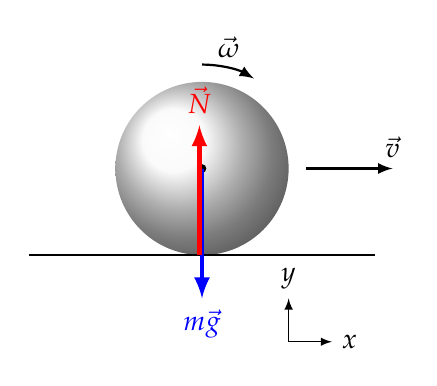
\begin{tikzpicture}[scale=1.1]
      \shade[ball color=gray!5](0,0) circle(1);
      \draw[thick](-2,-1)--(2,-1);
      \draw[thick,->](1.2,0)--(2.2,0) node[above]{$\vec v$};
      \draw[thick,->](0,1.2) arc(90:60:1.2) node[midway,above]{$\vec\omega$};
      \draw[->](1,-2)--(1.5,-2) node[right]{$x$};
      \draw[->](1,-2)--(1,-1.5) node[above]{$y$};
      \fill(0,0) circle(.05);
      \begin{scope}[->,ultra thick]
        \draw[blue](0,0)--(0,-1.5) node[below]{$m\vec g$};
        \draw[red](-.03,-1)--(-.03,.5) node[above]{$\vec N$};
      \end{scope}
    \end{tikzpicture}

    \column{.65\textwidth}
    \begin{itemize}
    \item Assumptions:
      \begin{itemize}
      \item Both the sphere and the surface are both perfectly rigid (they
        do not deform)
      \item The sphere and the surface are both perfectly smooth without defects
        even at the microscopic level
      \end{itemize}
    \item There are only two forces acting on the sphere:
      \begin{itemize}
      \item Gravitational force $m\vec g$
      \item Normal force $\vec N$
      \item There is no friction
      \end{itemize}
    \end{itemize}
  \end{columns}
\end{frame}



\begin{frame}{Pure Rolling Problems}
  The free-body diagram is simple enough that we can see that:
  \begin{columns}
    \column{.65\textwidth}
    \begin{itemize}
    \item There is no net force, therefore the translational state ($\vec v$)
      of the sphere is constant

      \eq{-.35in}{
        \sum\vec F=\vec 0\quad\quad \vec v=\text{constant}
      }
      
    \item\vspace{-.25in} Neither gravity or normal force generate a torque
      about the center of mass, therefore there is no net torque, and the
      rotational state $\vec\omega$ is constant:

      \eq{-.35in}{
        \sum\vec\tau=\vec 0\quad\quad\vec\omega=\text{constant}
      }
    \item\vspace{-.1in}In \emph{theory}, this sphere will roll along with
      angular speed $\omega$ and speed $v=\omega R$ forever
    \end{itemize}

    \column{.35\textwidth}
    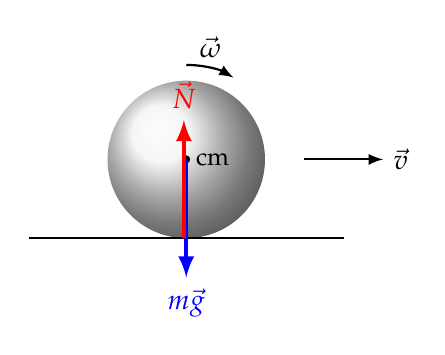
\begin{tikzpicture}
      \shade[ball color=gray!10](0,0) circle(1);
      \draw[thick](-2,-1)--(2,-1);
      \draw[thick,->](1.5,0)--(2.5,0) node[right]{$\vec v$};
      \draw[thick,->](0,1.2) arc(90:60:1.2) node[midway,above]{$\vec\omega$};
      \fill(0,0) circle(.05) node[right]{\small cm};
      \begin{scope}[->,ultra thick]
        \draw[blue](0,0)--(0,-1.5) node[below]{$m\vec g$};
        \draw[red](-.03,-1)--(-.03,.5) node[above]{$\vec N$};
      \end{scope}
    \end{tikzpicture}
  \end{columns}
\end{frame}



\begin{frame}{Reality: Rolling Resistance}
  In reality, the rolling sphere will slow down and eventually come to a stop,
  because \emph{nothing is perfectly rigid}: both the sphere and the surface
  deform when they make contact
  \begin{columns}
    \column{.7\textwidth}
    \begin{itemize}
    \item Example: a car's tires flatten when they make contact with the ground
    \item The normal force is larger in magnitude on the front side than on the
      other
    \item $N$ exerts both a horizontal force to slow down the sphere, as well
      as a torque to slow down its rotation
    \item The normal force does not point toward the CM because of the
      deformation.
    \end{itemize}

    \column{.3\textwidth}
    \vspace{.3in}
    \pic1{OAGZy}
  \end{columns}
\end{frame}




\begin{frame}{Rolling with Slipping on Rough Surface}
  What if the rolling sphere is slipping against the surface?
  \begin{columns}
    \column{.27\textwidth}
    \centering
    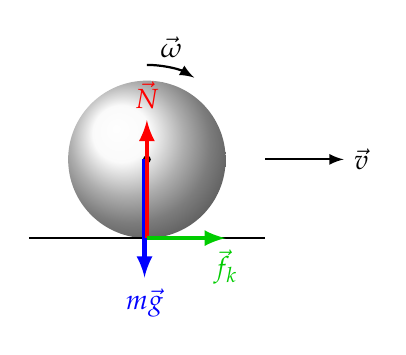
\begin{tikzpicture}
      \shade[ball color=gray!5](0,0) circle(1);
      \draw[thick](-1.5,-1)--(1.5,-1);
      \draw[thick,->](1.5,0)--(2.5,0) node[right]{$\vec v$};
      \draw[thick,->](0,1.2) arc(90:60:1.2) node[midway,above]{$\vec\omega$};
      \fill(0,0) circle(.05);
      \begin{scope}[->,ultra thick]
        \draw[blue](-0.03,0)--(-.03,-1.5) node[below]{$m\vec g$};
        \draw[red](0,-1)--(0,.5) node[above]{$\vec N$};
        \draw[green!80!black](0,-1)--(1,-1) node[below]{$\vec f_k$};
      \end{scope}
    \end{tikzpicture}

    \column{.73\textwidth}
    \begin{itemize}
    \item Slippage at the point of contact between the sphere and the flat
      surface
    \item There is \emph{kinetic} friction $f_k=\mu_kN$ in the $+\iii$
      direction (toward the right). The friction force generates:
      \begin{itemize}
      \item A net force $F_\text{net}$ in the $+\iii$ direction, toward the
        right
      \item A net torque $\tau_\text{net}$ in the $+\kkk$ direction, i.e.\
        counter clockwise
      \end{itemize}
    \end{itemize}
  \end{columns}
\end{frame}



\begin{frame}{Rolling with Slipping on Rough Surface}
  \begin{columns}
    \column{.27\textwidth}
    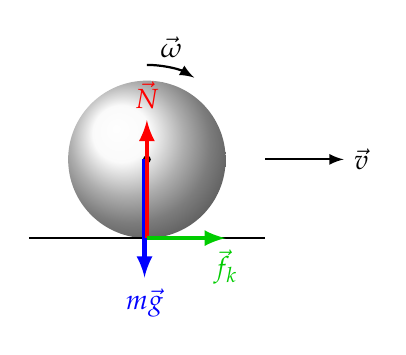
\begin{tikzpicture}
      \shade[ball color=gray!5](0,0) circle(1);
      \draw[thick](-1.5,-1)--(1.5,-1);
      \draw[thick,->](1.5,0)--(2.5,0) node[right]{$\vec v$};
      \draw[thick,->](0,1.2) arc(90:60:1.2) node[midway,above]{$\vec\omega$};
      \fill(0,0) circle(.05);
      \begin{scope}[->,ultra thick]
        \draw[blue](-0.03,0)--(-.03,-1.5) node[below]{$m\vec g$};
        \draw[red](0,-1)--(0,.5) node[above]{$\vec N$};
        \draw[green!80!black](0,-1)--(1,-1) node[below]{$\vec f_k$};
      \end{scope}
    \end{tikzpicture}

    \column{.73\textwidth}
    \begin{itemize}
    \item Kinetic friction $f_k$ causes the center of mass of the sphere to
      accelerate toward the right

      \eq{-.25in}{
        F_\text{net}=f_k=ma_\text{cm}
      }
      
    \item\vspace{-.2in}Since $f_k$ is constant, acceleration is also constant
      as well, as long as the sphere slips.
    \item e.g.: A car with its tires spinning on ice still has a small
      forward acceleration
    \item The acceleration of the center of mass is:

      \eq{-.25in}{
        a_\text{cm}=\mu_kg
      }
    \end{itemize}
  \end{columns}
\end{frame}



\begin{frame}{Rolling with Slipping on Rough Surface}
  \begin{columns}
    \column{.27\textwidth}
    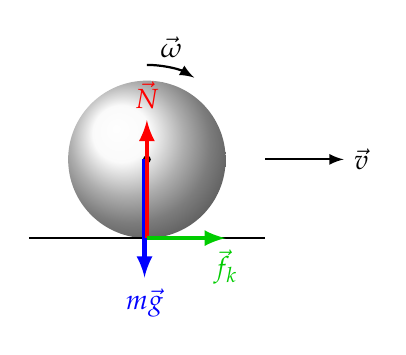
\begin{tikzpicture}
      \shade[ball color=gray!5](0,0) circle(1);
      \draw[thick](-1.5,-1)--(1.5,-1);
      \draw[thick,->](1.5,0)--(2.5,0) node[right]{$\vec v$};
      \draw[thick,->](0,1.2) arc(90:60:1.2) node[midway,above]{$\vec\omega$};
      \fill(0,0) circle(.05);
      \begin{scope}[->,ultra thick]
        \draw[blue](-0.03,0)--(-.03,-1.5) node[below]{$m\vec g$};
        \draw[red](0,-1)--(0,.5) node[above]{$\vec N$};
        \draw[green!80!black](0,-1)--(1,-1) node[below]{$\vec f_k$};
      \end{scope}
    \end{tikzpicture}

    \column{.73\textwidth}
    \begin{itemize}
    \item The constant net torque in the $+\kkk$ (counter clockwise) direction
      generates a constant angular acceleration (because $f_k$ is constant)

      \eq{-.25in}{
        \tau_\text{net}=f_kR=I\alpha
      }
    \item The angular acceleration causes the angular speed $\omega$ to
      decrease over time
    \item The angular acceleration in the $+\kkk$ direction:

      \eq{-.15in}{
        \alpha=\frac{\textcolor{green!80!black}{f_k}R}{\textcolor{purple}{I}}
        =\frac
        {\textcolor{green!80!black}{\mu_kmg}R}
        {\textcolor{purple}{\frac25mR^2}}
        =\frac{5\mu_kg}{2R}
      }
    \end{itemize}
  \end{columns}
\end{frame}



\begin{frame}{Rolling with Slipping on Rough Surface}
  \begin{columns}
    \column{.27\textwidth}
    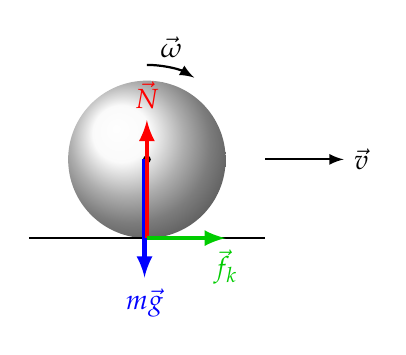
\begin{tikzpicture}
      \shade[ball color=gray!5](0,0) circle(1);
      \draw[thick](-1.5,-1)--(1.5,-1);
      \draw[thick,->](1.5,0)--(2.5,0) node[right]{$\vec v$};
      \draw[thick,->](0,1.2) arc(90:60:1.2) node[midway,above]{$\vec\omega$};
      \fill(0,0) circle(.05);
      \begin{scope}[->,ultra thick]
        \draw[blue](-0.03,0)--(-.03,-1.5) node[below]{$m\vec g$};
        \draw[red](0,-1)--(0,.5) node[above]{$\vec N$};
        \draw[green!80!black](0,-1)--(1,-1) node[below]{$\vec f_k$};
      \end{scope}
    \end{tikzpicture}

    \column{.73\textwidth}
    \begin{itemize}
    \item Unlike the no-slip case where where angular acceleration is related
      to linear acceleration by the radius, i.e.\ $a=\alpha R$, in this case,
      there is \textbf{no relationship between $\alpha$ and $a$.}
    \item There is also no relationship between the velocity and the center
      of mass and the angular velocity
    \item The speed of the sphere $v$ increases, while the angular speed
      $\omega$ decreases, until\ldots
    \item When $v=\omega r$, the sphere stops slipping, and the problem returns
      to the no-slip case
    \end{itemize}
  \end{columns}
\end{frame}



\begin{frame}{Rolling on an Inclined Surface}
  For a rigid and smooth sphere of radius $R$ rolling down a ramp of angle
  $\phi$ without slippage down a ramp of angle $\theta$.

  \vspace{.2in}
  \begin{columns}
    \column{.35\textwidth}
    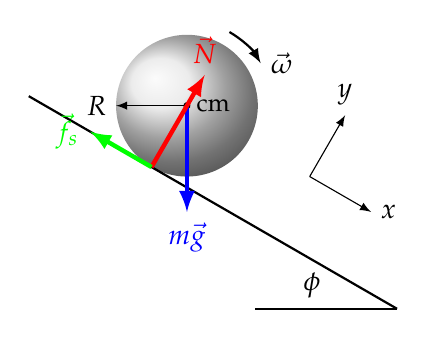
\begin{tikzpicture}[scale=.9]
      \begin{scope}[rotate=-30]
        \shade[ball color=gray!20](0,0) circle(1);
        \draw[thick](-2,-1)--(4,-1);
        \draw[->,rotate=30](0,0)--(-1,0) node[left]{$R$};
        \draw[thick,->](0,1.2) arc(90:60:1.2) node[right]{$\vec\omega$};
        \draw[->](2,0)--(3,0) node[right]{$x$};
        \draw[->](2,0)--(2,1) node[above]{$y$};
        \fill(0,0) circle(.05) node[right]{\small cm};
        \begin{scope}[->,ultra thick]
          \draw[blue,rotate=30](0,0)--(0,-1.5) node[below]{$m\vec g$};
          \draw[red](0,-1)--(0,.5) node[above]{$\vec N$};
          \draw[green](.0,-1)--(-1,-1) node[left]{$\vec f_s$};
        \end{scope}
        \begin{scope}[rotate around={30:(4,-1)}]
          \draw[thick](4,-1)--(2,-1) node[pos=.6,above]{$\phi$};
        \end{scope}
      \end{scope}
    \end{tikzpicture}

    \column{.65\textwidth}
    Three forces act on the sphere as it rolls down the ramp
    \begin{itemize}
    \item The weight ($mg$) of the sphere acts at the CM
    \item The normal force ($N$) acts at the point of contact
    \item The static friction ($f_s$) act at the point of contact
    \end{itemize}
    Only static friction generates a torque about the CM in the clockwise
    direction
    \begin{itemize}
    \item If $f_s$ is not present, there would have been nothing that causes
      the sphere to rotate.
    \end{itemize}
  \end{columns}
\end{frame}



\begin{frame}{Rolling on an Inclined Surface}
  \begin{columns}
    \column{.33\textwidth}
    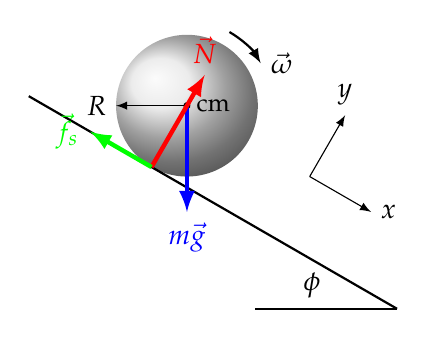
\begin{tikzpicture}[scale=.9]
      \begin{scope}[rotate=-30]
        \shade[ball color=gray!20](0,0) circle(1);
        \draw[thick](-2,-1)--(4,-1);
        \draw[->,rotate=30](0,0)--(-1,0) node[left]{$R$};
        \draw[thick,->](0,1.2) arc(90:60:1.2) node[right]{$\vec\omega$};
        \draw[->](2,0)--(3,0) node[right]{$x$};
        \draw[->](2,0)--(2,1) node[above]{$y$};
        \fill(0,0) circle(.05) node[right]{\small cm};
        \begin{scope}[->,ultra thick]
          \draw[blue,rotate=30](0,0)--(0,-1.5) node[below]{$m\vec g$};
          \draw[red](0,-1)--(0,.5) node[above]{$\vec N$};
          \draw[green](.0,-1)--(-1,-1) node[left]{$\vec f_s$};
        \end{scope}
        \begin{scope}[rotate around={30:(4,-1)}]
          \draw[thick](4,-1)--(2,-1) node[pos=.6,above]{$\phi$};
        \end{scope}
      \end{scope}
    \end{tikzpicture}

    \column{.67\textwidth}
    To solve this problem, there are three dynamics equations:
    \vspace{-.4in}{\Large
      \begin{align*}
        \sum F_x&=mg\sin\theta-f_s=ma\\
        \sum F_y&=N-mg\cos\theta=0\\
        \sum\tau &=Rf_s=I\alpha
      \end{align*}
    }
    
    \vspace{-.2in}At this point, static friction $f_s$ is \emph{not} known.
    The coefficient of static friction ($\mu_s$) only tells us the
    \emph{maximum} static friction, not the \emph{actual} friction. (We will
    instead use it to check if the answer makes sense.)
  \end{columns}
\end{frame}



\begin{frame}{Rolling on an Inclined Surface}
  \begin{columns}
    \column{.33\textwidth}
    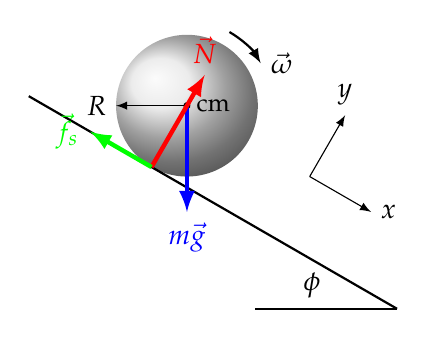
\begin{tikzpicture}[scale=.9]
      \begin{scope}[rotate=-30]
        \shade[ball color=gray!20](0,0) circle(1);
        \draw[thick](-2,-1)--(4,-1);
        \draw[->,rotate=30](0,0)--(-1,0) node[left]{$R$};
        \draw[thick,->](0,1.2) arc(90:60:1.2) node[right]{$\vec\omega$};
        \draw[->](2,0)--(3,0) node[right]{$x$};
        \draw[->](2,0)--(2,1) node[above]{$y$};
        \fill(0,0) circle(.05) node[right]{\small cm};
        \begin{scope}[->,ultra thick]
          \draw[blue,rotate=30](0,0)--(0,-1.5) node[below]{$m\vec g$};
          \draw[red](0,-1)--(0,.5) node[above]{$\vec N$};
          \draw[green](.0,-1)--(-1,-1) node[left]{$\vec f_s$};
        \end{scope}
        \begin{scope}[rotate around={30:(4,-1)}]
          \draw[thick](4,-1)--(2,-1) node[pos=.6,above]{$\phi$};
        \end{scope}
      \end{scope}
    \end{tikzpicture}

    \column{.67\textwidth}
    For non-slip case, angular and translational acceleration are related using
    relative motion:

    \eq{-.3in}{ a=\alpha R}
    
    \vspace{-.22in}Solving for the static friction:

    \eq{-.15in}{
      f_s=\frac{I\alpha}R=
      \frac25mR^2\cdotp\frac aR\cdotp\frac1R=\frac25ma
    }

    It is substituted into the force equation in the $\iii$ direction to
    solve for the acceleration of the CM down the ramp:

    \eq{-.2in}{
        mg\sin\theta-\frac25 ma=ma
    }
  \end{columns}
\end{frame}


\begin{frame}{Rolling on an Inclined Surface}
  \begin{columns}
    \column{.33\textwidth}
    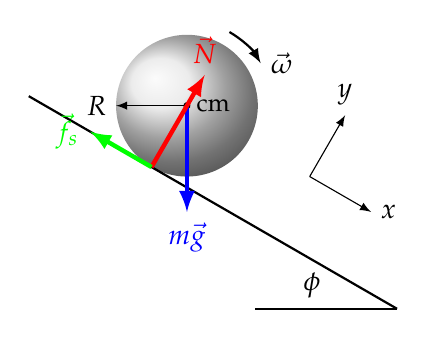
\begin{tikzpicture}[scale=.9]
      \begin{scope}[rotate=-30]
        \shade[ball color=gray!20](0,0) circle(1);
        \draw[thick](-2,-1)--(4,-1);
        \draw[->,rotate=30](0,0)--(-1,0) node[left]{$R$};
        \draw[thick,->](0,1.2) arc(90:60:1.2) node[right]{$\vec\omega$};
        \draw[->](2,0)--(3,0) node[right]{$x$};
        \draw[->](2,0)--(2,1) node[above]{$y$};
        \fill(0,0) circle(.05) node[right]{\small cm};
        \begin{scope}[->,ultra thick]
          \draw[blue,rotate=30](0,0)--(0,-1.5) node[below]{$m\vec g$};
          \draw[red](0,-1)--(0,.5) node[above]{$\vec N$};
          \draw[green](.0,-1)--(-1,-1) node[left]{$\vec f_s$};
        \end{scope}
        \begin{scope}[rotate around={30:(4,-1)}]
          \draw[thick](4,-1)--(2,-1) node[pos=.6,above]{$\phi$};
        \end{scope}
      \end{scope}
    \end{tikzpicture}

    \column{.67\textwidth}
    The acceleration of the center of mass is therefore:

    \eq{-,2in}{
      a=\frac57 g\sin\theta
    }

    \vspace{-.1in}Compare this to an object \emph{sliding} without friction
    down the same ramp, which is higher than the pure rolling case.
    
    \eq{-.25in}{
      a=g\sin\theta
    }
    
%The simplest explanation is that some of the gravitational potential energy is
%converted to both translational and rotational kinetic energies, while for the
%sliding case, all of the potential energy is converted into translational
%kinetic energy.
%If this is indeed the case, it means that the sphere will actually slip while
%rolling down the ramp, and the friction at the contact point is in fact kinetic
%friction.

    \vspace{-.2in}If the sphere starts from rest, the speed of the sphere when
    it reaches the bottom of the ramp, a distance $d$ away, would be:

    \eq{-.2in}{
      v=\sqrt{2ad}=\sqrt{\frac{10}7gd\sin\theta}
    }

%There is, of course, one ``sanity check'' that must be done, that is to make
%sure that the friction calculated in Eq.~\ref{f_s} has not exceeded the maximum
%static friction, given by
%\begin{equation}
%  f_s\leq\mu_s N
%  \label{maxf}
%\end{equation}
%Combining the expression for $f_s$ in Eq.~\ref{f_s}, the acceleration in
%Eq.~\ref{pure-roll-accel}, and the normal force on an incline, Eq.~\ref{maxf}
%becomes:
%\begin{align}
%  f_s&\leq\mu_sN\\
%  \frac27mg\sin\theta&\leq\mu_smg\cos\theta\\
%  \frac27\tan\theta&\leq\mu_s
%\end{align}
%If the ramp angle is too steep, then the friction will transition from static
    %to kinetic, which is a much more difficult problem.

  \end{columns}
\end{frame}



\section{Work \& Energy in Rotational Motion}

\begin{frame}{Mechanical Work}
  For translational motion, mechanical work is defined as

  \eq{-.2in}{
    W_t=\int_{x_1}^{x_2}\vec F\cdot\dl\vec x
  }

  For rotational motion, mechanical work is defined similarly as:

  \eq{-.2in}{
    \boxed{
      W_r=\int_{\theta_1}^{\theta_2}\tau\dl\theta
    }
  }

  The work-energy theorem still applies to rotational motion, i.e.;

  \eq{-.25in}{
    W_r=\Delta K_r
  }
\end{frame}



\begin{frame}{Rotational Kinetic Energy}
  To find the kinetic energy of a rotating system of particles (discrete number
  of particles, or continuous mass distribution), we sum the
  kinetic energies of the individual particles:
    
  \eq{-.1in}{
    K_r=\sum_i\frac12m_iv_i^2=\sum\frac12m_i(r_i\omega)^2
    =\frac12\left(\sum_i m_ir_i^2\right)\omega^2
  }
  
  It's no surprise that rotational kinetic energy is given by:
  
  \eq{-.2in}{
    \boxed{K_r=\frac12I\omega^2}
  }
\end{frame}



\begin{frame}{Kinetic Energy of a Rotating System}
  The total kinetic energy of a rotating system is the sum of its translational
  and rotational kinetic energies at its center of mass:

  \eq{-.2in}{
    \boxed{K=K_t+K_r=\frac12mv_\text{cm}^2+\frac12I_\text{cm}\omega^2}
  }
  
  In this case, $I_\text{cm}$ is calculated at the center of
  mass. For simple problems, we only need to compute rotational kinetic energy
  at the pivot:

  \eq{-.2in}{
    \boxed{K=\frac12I_\text{P}\omega^2}
  }
  
  In this case, the $I_\text{P}$ is calculated at the pivot.
  \textbf{IMPORTANT:} $I_\text{cm}\neq I_\text{P}$
\end{frame}



\begin{frame}{Parallel Axis Theorem}
  \begin{columns}
    \column{.35\textwidth}
    \pic{1}{Steiner}
    
    \column{.65\textwidth}
    The \textbf{parallel axis theorem} relates the moment of inertia of an
    object along two different but parallel axis by:

    \eq{-.2in}{
      \boxed{I=I_\text{cm}+md^2}
    }
  \end{columns}
\end{frame}
\end{document}
